\documentclass[journal]{IEEEtran}

\usepackage{amsmath,amssymb,amsfonts}
\usepackage{algorithm}
\usepackage{algorithmic}
\usepackage{graphicx}
\graphicspath{{../Paper/figures/}}
\usepackage{textcomp}
\usepackage{xcolor}
\usepackage{booktabs}
\usepackage{multirow}
\usepackage{url}
\usepackage[hidelinks,hypertexnames=false]{hyperref}
\usepackage{cite}

% Keep the journal layout within 12 pages without shrinking figure content.
\setlength{\textfloatsep}{7pt plus 1pt minus 2pt}
\setlength{\floatsep}{6pt plus 1pt minus 2pt}
\setlength{\intextsep}{6pt plus 1pt minus 2pt}

\newtheorem{definition}{Definition}
\newtheorem{problem}{Problem}

\begin{document}

\title{ContractKV: Certified Prompt Compilation for\\Transactional Prefix Reuse in Multi-Tenant LLM Services}

\author{Bin~Zhou and Xi~Cao,~\IEEEmembership{Member,~IEEE}
\thanks{B. Zhou is with the College of Information Science and Technology, Beijing University of Chemical Technology, Beijing 102218, China (e-mail: 2025200800@buct.edu.cn).}
\thanks{X. Cao is with the College of Information Science and Technology, Beijing University of Chemical Technology, Beijing 102218, China (e-mail: caoxi@buct.edu.cn).}
\thanks{Corresponding author: Xi Cao.}
}

\markboth{IEEE Transactions on Services Computing}%
{ContractKV: Certified Prompt Layout Compilation}

\maketitle

\begin{abstract}
Prefix caching accelerates LLM serving only when reusable tokens form a contiguous physical prefix. In repeated agent, retrieval, and code services, 85.0\% of prompt tokens are stable, yet native automatic prefix caching recovers only 2.4\%. We present ContractKV, a service control plane that converts this latent stability into governed physical reuse. A contract-aware compiler constructs dependency-valid stable-prefix layouts; prospective qualification and strict teacher-forced attestation admit only behaviorally supported routes; signed, versioned certificates bind model, runtime, template, policy, authorization, and lifecycle identity; and Prefix-Selective Transactional Promotion makes only exact-LCP, block-aligned stable state visible to the shared cache. A frozen net-benefit gate retains raw order outside profitable scopes, while service-template certificates amortize in-engine verification across authorized tenants. On vLLM~0.10.2, four configurations from three model families reduce all-workflow mean TTFT by 29.41--44.69\%, including raw fallback and measured verification charges. In a five-repeat Llama-3.1-8B comparison, ContractKV reduces mean TTFT by 29.16\% over native APC, compared with 26.96\% for CacheBlend over its matched runtime. Observed material paired task-score regressions are 0.089\% overall and 0/1{,}125 among admitted compiled requests; both overall events occur on raw fallback and reproduce under raw-only control, whereas CacheBlend exhibits a 9.956\% regression rate. In an independent same-engine Qwen3-8B closure, template-scoped ContractKV reduces mean TTFT by 92.90\% after charging registration wall time. Across the 25-tenant load sweep it improves 500-ms SLO goodput by 4.81$\times$, and at 80 tenants peak KV-block occupancy falls by 72\%. Across live fault probes and 325{,}000 transactional stress operations, no aborted transaction publishes compiled blocks.
\end{abstract}

\begin{IEEEkeywords}
KV cache, LLM inference serving, prefix caching, service-level objectives, multi-tenant consolidation, behavioral certification, transactional reuse.
\end{IEEEkeywords}

% ============================================================
\section{Introduction}
\label{sec:introduction}
% ============================================================

Multi-tenant LLM inference services consolidate diverse agent, retrieval, and tool-augmented workflows onto shared GPU infrastructure, where service-level objectives (SLOs) on time-to-first-token (TTFT) and goodput govern deployment economics~\cite{vllm2023,sglang2024}. We target deployments in which authorized tenants repeatedly consume a stable service template and its prefix remains resident often enough to amortize certification. Because prefill work grows with prompt length, modern serving engines widely deploy prefix caching: they physically reuse the key-value (KV) states of token-identical prefixes~\cite{vllm2023,sglang2024}, lowering TTFT without changing model semantics.

Prefix caching nevertheless has a structural blind spot in increasingly common structured services. Agent pipelines~\cite{react2023}, retrieval-augmented generation (RAG), and multi-turn tool use~\cite{toolformer2023} compose prompts from heterogeneous segments---system instructions, retrieved documents, repository context, observations, and conversation state---whose application order need not match their reuse potential. One changed observation between two stable segments terminates the physical prefix even when all downstream stable content is byte-identical. Across five representative service families, stable content accounts for 78--91\% of prompt tokens, whereas native caching recovers under 3\% in raw arrival order. The resulting gap between an \emph{application-declared byte-stable working set} and \emph{physical prefix continuity} creates redundant prefill work that compounds with context length and tenant fan-out.

Moving stable segments ahead of volatile ones can expose this reuse, but prefix maximization alone is not an admissible service policy. Segment order encodes data, causal, and positional dependencies; even a dependency-valid permutation can change position-sensitive generation. Once transformed KV state becomes visible in a shared cache, a behavioral error, stale identity, or scope mismatch can affect subsequent tenants.

Recent non-prefix reuse systems selectively fuse or recompute moved segments~\cite{cacheblend2025,sparsex2026}. They expand the reuse space but do not by themselves answer a service-level question: \emph{when may transformed state become visible to other requests?} A safe service must validate dependencies, bind model-backed evidence to runtime and authorization identity, revoke it across lifecycle changes, and prevent failed verification from partially publishing shared state. ContractKV therefore treats compiled KV as a versioned service object, not only a performance artifact.

We present \textsc{ContractKV}, a compile--attest--commit control plane for multi-tenant prefix reuse. (1)~A \emph{Contract-Aware Layout Compiler} (CALC) constructs a bounded ladder of dependency-valid layouts with progressively longer stable prefixes. (2)~\emph{Scoped Behavioral Certification} uses prospective qualification, strict teacher-forced token-path agreement, and signed versioned identity to admit only supported model--workflow--layout routes. (3)~\emph{Prefix-Selective Transactional Promotion} (PSTP) keeps candidate state private and makes only verified, exact-LCP, block-aligned stable blocks visible at one scheduler-thread linearization point. (4)~A frozen \emph{net-benefit gate} retains raw order outside profitable scopes, while a service-template certificate amortizes one deployment attestation across authorized tenants. Failure, identity mismatch, scope conflict, timeout, or profitability rejection publishes no compiled state.

We evaluate \textsc{ContractKV} on vLLM~0.10.2 using Qwen3-8B, Qwen3-14B (TP=2), Mistral-7B-Instruct-v0.3, and Llama-3.1-8B. Across five workflows, all four configurations reduce all-workflow mean TTFT by 29.41--44.69\% after accounting for direct L0 routing, runtime fallback, and measured verification charges. Under the same frozen RULER scope, Qwen, Mistral, and Llama converge to 85.97--87.41\% reduction. In a five-repeat Llama comparison, ContractKV achieves a 29.16\% matched-baseline reduction, compared with 26.96\% for CacheBlend, while reducing observed material paired regressions from 9.956\% to 0.089\%; no such regression occurs among 1{,}125 admitted compiled requests. An independent same-engine verifier closure charges all template-registration wall time and reduces Qwen3-8B mean TTFT by 92.90\%. Across the primary load sweep, ContractKV improves 500-ms SLO goodput by 4.81$\times$, and at 80 tenants reduces peak KV-block occupancy by 72\%. Live fault probes, signed-binding tests, and 325{,}000 state-machine transactions report no partial publication or stale-scope admission.

This paper makes the following contributions:
\begin{itemize}
    \item We formulate \emph{certified prompt compilation} for structured LLM services. An operator-registered manifest defines segment stability, separators, dependencies, authorization, and expected fan-out; undeclared tenant content defaults to private. CALC constructs a bounded ladder of dependency-valid native-prefix layouts.
    \item We introduce scoped behavioral certification and service-template certificates. Strict token-path attestation is bound to model/runtime identity, template version, policy, authorization domain, and lifecycle epoch, enabling deployment-level amortization without sharing private suffix state.
    \item We design PSTP, which keeps candidate KV state outside the shared prefix index until a valid commit and atomically publishes only the exact-LCP, block-aligned stable subset. Abort, timeout, duplicate, identity, and scope conflicts publish no compiled blocks.
    \item We implement ContractKV in the vLLM V1 scheduler and evaluate it across four model configurations, five task families, direct non-prefix-reuse baselines, same-engine verification, open-loop SLO workloads, 80-tenant consolidation, signed binding, live fault injection, and 325{,}000 transactional stress operations.
\end{itemize}


% ============================================================
\section{Background and Motivation}
\label{sec:background}
% ============================================================

\subsection{Prefix Caching in LLM Serving}

Modern LLM serving engines decompose transformer~\cite{transformer2017} inference into a \textbf{prefill} phase---which computes key-value (KV) states for prompt tokens via optimized attention kernels~\cite{flashattention2022}---and an autoregressive \textbf{decode} phase. Schedulers~\cite{orca2022,sarathi2024} interleave both phases across concurrent requests. For long contexts, many deployments enable \emph{prefix caching}: when a token sequence shares a prefix with resident state, the engine reuses those KV blocks and computes only the suffix~\cite{vllm2023,sglang2024}.

Formally, let $\mathbf{t} = (t_1, \ldots, t_n)$ be a request's token sequence and $\mathcal{R}$ the set of resident KV states in the cache. The engine identifies the longest prefix match
\begin{equation}
  k^* = \max\{k : (t_1, \ldots, t_k) \in \mathcal{R}\},
\end{equation}
reuses $k^*$ blocks, and computes only the remaining $n - k^*$ tokens. Under \emph{automatic prefix caching} (APC) in vLLM~\cite{vllm2023} or \emph{RadixAttention} in SGLang~\cite{sglang2024}, this matching is performed at block granularity $B$ (typically 16 tokens), yielding physical reuse of $\lfloor k^*/B \rfloor$ blocks.

This mechanism is highly effective for \emph{homogeneous} workloads---batch inference over identical system prompts, or multi-turn conversations where each turn appends to a growing prefix. In these settings, prefix reuse rates exceed 90\% and TTFT reductions are substantial.

\subsection{The Structural Blind Spot}

Production LLM \emph{services}, however, are increasingly \emph{structured}: a single request composes multiple semantic segments---system instructions, retrieved documents, repository context, tool observations, and conversation state---whose physical ordering in the prompt is dictated by application logic rather than reuse potential. We term the resulting inefficiency the \textbf{structural blind spot}: the cache can only exploit \emph{physical prefix continuity}, but the \emph{semantic working set} that is actually reusable is distributed across non-contiguous positions.

\smallskip
\noindent\textbf{Motivating measurement.}
We instrumented five representative service families (RULER, HotpotQA, NarrativeQA, Qasper, RepoBench) with 25 source-group-disjoint sessions each, 10 turns per session. Each session freezes source context into an operator-registered template and derives its later query/observation turns from a SHA-frozen trace manifest. For each request we compute:
\begin{itemize}
  \item \emph{Stable-token ratio} $\rho_s$: fraction of prompt tokens belonging to segments that remain byte-identical across turns within the same session.
  \item \emph{Native prefix recovery} $\rho_p$: fraction of stable tokens actually recovered by the engine's native APC under raw arrival order.
\end{itemize}

\noindent Table~\ref{tab:motivation} reports the results. The gap is stark: stable content constitutes 78--91\% of prompt tokens, yet native prefix caching recovers fewer than 3\% of this available reuse. The root cause is architectural: a single mutable segment (e.g., a tool observation) inserted between two large stable segments \emph{fractures} the physical prefix, rendering all downstream stable content invisible to the cache despite being computationally identical.

\begin{table}[t]
\centering
\caption{Structural blind spot: stable content vastly exceeds physical prefix recovery across five service families (Qwen3-8B, 10-turn sessions).}
\label{tab:motivation}
\small
\begin{tabular}{@{}lcc@{}}
\toprule
\textbf{Service Family} & \textbf{Stable Ratio $\rho_s$} & \textbf{Native Recovery $\rho_p$} \\
\midrule
RULER (NIAH)        & 91.2\% & 2.8\% \\
HotpotQA            & 82.4\% & 2.1\% \\
NarrativeQA         & 78.6\% & 1.9\% \\
Qasper              & 84.1\% & 2.4\% \\
RepoBench           & 88.7\% & 2.6\% \\
\midrule
\textbf{Mean}       & \textbf{85.0\%} & \textbf{2.4\%} \\
\bottomrule
\end{tabular}
\end{table}

\begin{figure*}[t]
\centering
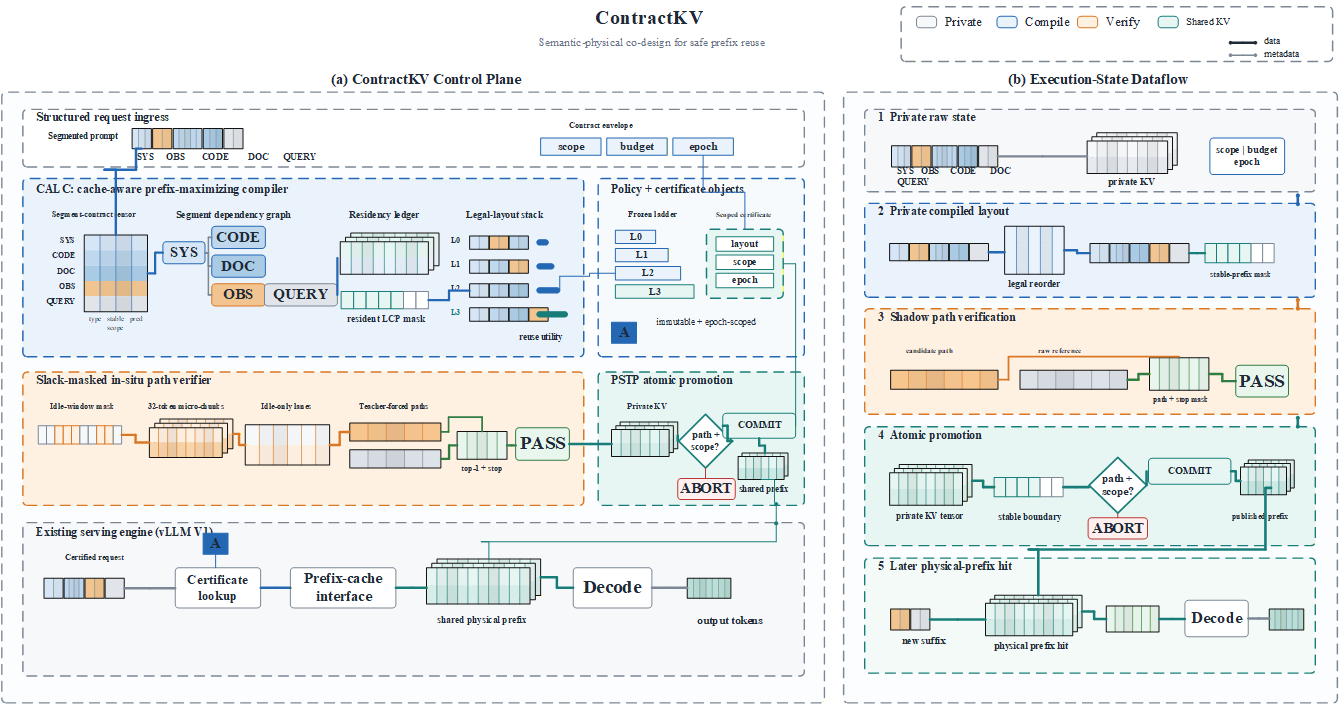
\includegraphics[width=\textwidth]{fig1_contractkv_visio.png}
\caption{ContractKV control-plane architecture and execution-state dataflow. (a) CALC combines segment contracts, the SDG, resident-prefix state, and qualification metadata; the verifier and PSTP publish only behaviorally certified compiled blocks into the vLLM cache domain. Solid arrows carry requests or KV state, whereas dashed arrows carry policy and certificate metadata. (b) A selected request evolves from private raw tokens to a private compiled layout, shadow verification, atomic promotion, and a later physical-prefix hit. A failed promotion discards only candidate compiled state; the raw-order path may populate native APC state as in unmodified vLLM.}
\label{fig:architecture}
\end{figure*}

This gap appears whenever an application interleaves byte-stable context with per-request observations and revisits the same authorized template. The degree of benefit is workload dependent: reuse must survive declared dependencies, behavioral admission, and cache residency. When those conditions hold, each unrecovered stable token incurs redundant prefill work, occupies scheduler slots, and consumes TTFT budget.

\subsection{Why Naive Reordering Is Inadmissible}

A natural response is to \emph{reorder} stable segments ahead of volatile ones, exposing a longer physical prefix. While this recovers reuse in principle, it introduces two correctness hazards that make unconstrained reordering unacceptable in a shared serving system:

\smallskip
\noindent\textbf{Hazard 1: Dependency violation.}
Segment order encodes semantic dependencies. A tool observation may depend on a preceding system instruction; a code completion requires repository context before the query; a chronological agent history must preserve causal ordering. Arbitrary permutation violates these constraints, producing prompts that are cache-friendly but \emph{semantically ill-formed}.

\smallskip
\noindent\textbf{Hazard 2: Behavioral drift.}
Even when all dependencies are satisfied, a reordered prompt may shift the model's output distribution. Transformer attention is position-sensitive: moving a segment from position $i$ to position $j$ changes its attention pattern and can alter generation. Publishing an unverified reordered prefix into a shared cache makes this behavioral consequence \emph{visible to all subsequent requests}---a silent, system-wide correctness risk with no rollback mechanism.

\smallskip
\noindent\textbf{The fundamental tension.}
Exploiting structural reuse requires layout control; safe layout control requires verification; and reusable verification requires explicit scope and transactional publication. To our knowledge, no prior system jointly provides these properties. Figure~\ref{fig:architecture} shows how ContractKV connects the compiler, certifier, and cache publication path.

% ============================================================
\section{Service Model and Problem Formulation}
\label{sec:formulation}
% ============================================================

We now formalize the structured-prompt prefix-maximization problem that ContractKV solves. The formulation proceeds in three layers: a segment model with typed stability annotations, a dependency-constrained layout optimization objective, and a multi-tenant service-template abstraction.

\subsection{Structured Request and Segment Model}

\begin{definition}[Structured Request]
A \textbf{structured request} $r$ is an ordered tuple of \emph{semantic segments}
\begin{equation}
  r = (s_1, s_2, \ldots, s_m), \quad s_i = (\textit{id}_i,\; \tau_i,\; \sigma_i,\; \mathbf{c}_i),
\end{equation}
where $\textit{id}_i$ is a unique segment identifier, $\tau_i \in \mathcal{T} = \{\textsc{Stable}, \textsc{Mutable}, \textsc{Query}\}$ is the \textbf{stability type}, $\sigma_i$ is a content hash, and $\mathbf{c}_i$ is the token sequence of segment $s_i$. Stability types and legal dependencies are supplied by an operator-registered service-template manifest; unregistered tenant inputs default to private mutable or query segments.
\end{definition}

\noindent\textbf{Trust boundary.} \textsc{Stable} is a privileged type granted only by an operator-registered, versioned service manifest. Request-time tenant input, tool output, request identifiers, and undeclared segments default to private \textsc{Mutable} or \textsc{Query} state and cannot acquire shareable status through request metadata. The manifest binds segment boundaries, frozen separators, content hashes, dependency edges, and the authorization domain.

The stability type captures the segment's reuse potential within a service session:
\begin{itemize}
  \item \textsc{Stable}: content is byte-identical across all turns in the session (system prompts, retrieved documents, repository context). These segments constitute the \emph{reusable working set}.
  \item \textsc{Mutable}: content changes across turns but follows a predictable lifecycle (tool observations, intermediate results). These segments \emph{fracture} prefix continuity.
  \item \textsc{Query}: the per-turn user query or action. Always unique; never reusable.
\end{itemize}

\noindent Let $L(r) = \sum_{i=1}^{m} |\mathbf{c}_i|$ denote the total prompt length and $L_s(r) = \sum_{i:\tau_i = \textsc{Stable}} |\mathbf{c}_i|$ the stable-token length. The \emph{structural reuse potential} is $\rho_s(r) = L_s(r) / L(r)$.

\subsection{Segment Dependency Graph}

\begin{definition}[Segment Dependency Graph]
The \textbf{segment dependency graph} (SDG) of a request $r$ is a directed acyclic graph $G_r = (V, E, \lambda)$ where:
\begin{itemize}
  \item $V = \{s_1, \ldots, s_m\}$ is the set of segment vertices;
  \item $E \subseteq V \times V$ is the set of \emph{typed dependency edges}---$(s_i, s_j) \in E$ indicates that segment $s_i$ must precede $s_j$ in any valid layout;
  \item $\lambda: E \rightarrow \{\textsc{Data}, \textsc{Causal}, \textsc{Positional}\}$ labels each edge with its dependency type.
\end{itemize}
\end{definition}

Edge types carry distinct semantics: \textsc{Data} edges encode information flow (a tool result depends on its input); \textsc{Causal} edges encode temporal ordering (turn $k$ depends on turn $k{-}1$); \textsc{Positional} edges encode model-specific sensitivity (instruction must precede query). The SDG is constructed from the operator-registered manifest's segment boundaries, content hashes, and dependency edges; it does not infer shareability from tenant-provided metadata.

\begin{definition}[Layout]
A \textbf{layout} $\pi$ of request $r$ is a permutation of $V$ such that $\pi$ is a \emph{topological ordering} of $G_r$:
\begin{equation}
  \forall (s_i, s_j) \in E: \quad \text{pos}_\pi(s_i) < \text{pos}_\pi(s_j).
\end{equation}
The set of all valid layouts is $\Pi(G_r) = \{\pi : \pi \text{ is a topological order of } G_r\}$.
\end{definition}

\subsection{Layout Validity and Prefix Maximization}

Given a layout $\pi$, the \emph{compiled prompt} is the concatenation $\mathbf{c}_\pi = \mathbf{c}_{\pi(1)} \| \mathbf{c}_{\pi(2)} \| \cdots \| \mathbf{c}_{\pi(m)}$. Let $q(\pi)$ be the number of leading stable segments and $P(\pi)$ their token length:
\begin{equation}
\begin{aligned}
q(\pi)&=\max\{q:\forall j\leq q,\;\tau_{\pi(j)}=\textsc{Stable}\},\\
P(\pi)&=\sum_{j=1}^{q(\pi)}|\mathbf{c}_{\pi(j)}|.
\end{aligned}
\end{equation}
The physical reuse at block granularity $B$ is $\lfloor P(\pi) / B \rfloor$ blocks.

\begin{problem}[Dependency-Constrained Prefix Maximization]
\label{prob:dcpx}
Given a structured request $r$ with SDG $G_r$, resident state $\mathcal{R}$, and a finite compiler ladder $\Pi_L(G_r)=\{\pi_0,\ldots,\pi_K\}\subseteq\Pi(G_r)$, maximize block-aligned reuse over the frozen ladder:
{\small
\begin{align}
  \pi^*=\arg\max_{\pi\in\Pi_L(G_r)} &\ \textit{reuse}_B(\pi,\mathcal{R}) \label{eq:objective} \\
  \text{s.t.} \quad & \textit{BehavioralAdmission}(\pi,r;\theta,C)=\textsc{Pass}, \label{eq:behav}\\
  & \textit{ScopeValid}(r,C)=1, \label{eq:scope}\\
  & \textit{BenefitGate}(\pi,\Theta)=\textsc{Pass}. \label{eq:benefit}
\end{align}
}
Here $\pi_0$ is raw order and each ladder member is dependency-valid by construction. The compiler maximizes reuse only within the set admitted by three frozen controls: behavioral attestation, certificate scope, and prospective net benefit. The implementation takes the first passing member in frozen high-to-low order; resident state is a reuse witness and admission input, not an online optimizer of construction order. The 0.03 task-score threshold used in evaluation is a separate post-hoc quality gate, not the admission tolerance.
\end{problem}

\noindent Exact optimization would search dependency-valid topological orders while evaluating a model-backed behavioral predicate. ContractKV instead uses a bounded \emph{layout ladder} (Section~\ref{sec:calc}); the ledger rejects candidates that expose no resident block and certification evaluates the remaining frozen-order candidates. We do not rely on an unproven complexity classification for this search problem.

\subsection{Service-Template Model}

In multi-tenant LLM serving, multiple tenants issue requests against a shared stable context. We abstract this as:

\begin{definition}[Service Template]
A \textbf{service template} $\Theta = (\mathbf{S}, \mathcal{A}, \mathcal{P}, \mathcal{M}, F)$ consists of:
\begin{itemize}
  \item $\mathbf{S} = (s_1, \ldots, s_k)$: the ordered set of \textsc{Stable} segments shared across all authorized tenants;
  \item $\mathcal{A} = \{a_1, \ldots, a_N\}$: the set of authorized tenant identifiers;
  \item $\mathcal{P}$: the frozen policy governing verification, layout selection, and certificate issuance;
  \item $\mathcal{M}$: an operator-registered manifest containing immutable segment boundaries, dependency edges, separators, and authorization domain.
  \item $F$: an operator-declared reuse commitment (expected authorized future fan-out) used by the frozen benefit gate.
\end{itemize}
\end{definition}

Each tenant $a_i$ appends private \textsc{Mutable} and \textsc{Query} segments to $\mathbf{S}$, forming a tenant-specific request $r_i = \mathbf{S} \| \mathbf{m}_i \| \mathbf{q}_i$. The \textbf{service locality} of a workload is the expected number of tenants sharing each template; higher locality implies greater amortization of verification cost and prefix-state residency.

The service-level objective extends Problem~\ref{prob:dcpx} to the multi-tenant setting: maximize aggregate SLO goodput (fraction of requests meeting a TTFT deadline $\Delta_{\text{SLO}}$) across all tenants, subject to unauthorized-reuse isolation (private suffix state is not shared across tenants) and certificate-scope admissibility.

\subsection{Safety and Isolation Invariants}

ContractKV enforces four design invariants in the implementation and validates their failure paths through source-level instrumentation and fault injection:

\smallskip
\noindent\textbf{(P1) Publication safety.}
No \emph{candidate compiled} KV state becomes visible in the shared prefix cache unless it has passed behavioral verification \emph{and} carries a valid certificate whose scope subsumes the current request:
\begin{equation}
  \textit{Visible}_{\rm compiled}(x) \implies \exists\, C: \textit{Valid}(C, x) \wedge C.\textit{status} = \textsc{Pass}.
\end{equation}

\noindent\textbf{(P2) Suffix isolation.}
The transactional commit boundary is block-aligned to the stable-prefix length and exact candidate--certificate token LCP; no \textsc{Mutable} or \textsc{Query} token is promoted:
\begin{equation}
\begin{aligned}
  L_{\rm lcp}&=\operatorname{LCP}(\mathbf{t}_{\rm cand},\mathbf{t}_{\rm cert}),\\
  L_{\rm commit}&=B\left\lfloor\frac{\min(L_s,L_{\rm cert},L_{\rm lcp})}{B}\right\rfloor,\\
  N_{\rm blocks}&=L_{\rm commit}/B.
\end{aligned}
\end{equation}
where $L_{\rm cert}$ is the prompt-prefix length authorized by attestation.

\noindent\textbf{(P3) Fail-closed semantics.}
Any verification failure, scope mismatch, timeout, or identity conflict aborts promotion with \emph{zero publication of candidate compiled state}. The request then resumes under raw order; assuming progress of the base engine, this fallback also preserves progress. Native APC may populate raw-order cache state exactly as in unmodified vLLM.

\noindent\textbf{(P4) Tenant isolation.}
For tenants $a_i \neq a_j$ under the same template $\Theta$, private observations, request identifiers, and candidate namespaces remain disjoint. Cross-tenant KV reuse is confined to the authorized stable prefix $\mathbf{S}$; this is a cache-state isolation claim, not a claim about the surrounding application's security boundary.

% ============================================================
\section{ContractKV Design}
\label{sec:design}
% ============================================================

ContractKV resolves Problem~\ref{prob:dcpx} through a four-stage pipeline---\emph{compile}, \emph{certify}, \emph{promote}, \emph{amortize}---that operates entirely within the serving engine's existing prefix-cache substrate. No hardware modification, custom kernel, or external oracle is required. We present each stage in turn.

% ------------------------------------------------------------
\subsection{Contract-Aware Layout Compiler}
\label{sec:calc}
% ------------------------------------------------------------

The \textbf{Contract-Aware Layout Compiler} (CALC) transforms request $r$ into a bounded ladder of dependency-valid candidates. ``Contract-aware'' is deliberate: cache residency informs benefit admission, while semantic dependencies, authorization, and frozen qualification determine legality. L0 is raw order. For Llama calibration, stable content is split into $K=16$ contiguous character-preserving units; L1/L2/L3 select 4/12/16 eligible units. A stable-priority topological sort moves units only as early as declared SDG edges permit, breaks ties by original index, inserts frozen separators, and requires full retokenization plus an exact rendered-prompt audit. Qwen and Mistral evaluate one full candidate, L3*, under the same certificate protocol; they do not claim separately calibrated L1/L2 semantics.

\smallskip
\noindent\textbf{Prospective qualification.}
For a new model, every family--level pair is evaluated on a source-disjoint development split. The highest level satisfying completion, future-turn quality, scope, output-length, physical-reuse, and suffix-isolation gates becomes the frozen family maximum. The eligible descent set, policy hash, and qualification hash are frozen \emph{before} the sealed held-out split is opened. Held-out outcomes never change the ladder or thresholds.

\smallskip
\noindent\textbf{Runtime descent and benefit admission.}
The compiler tries only levels in the frozen eligible descent set. Before verification, a frozen minimum-benefit rule rejects scopes without sufficient certified fan-out; each remaining candidate must add at least one reusable block and pass strict verification and scope validation. Any failed gate descends, eventually returning L0. Algorithm~1 is the implemented admission path.

\begin{algorithm}[t]
\footnotesize
\begin{algorithmic}[1]
\STATE Validate signed manifest; mark undeclared segments private
\STATE Split stable text into contiguous units; freeze separators
\STATE Build L0--L3 candidates by stable-priority topological sort
\STATE Break ties by original index; retokenize and audit each prompt
\IF{frozen benefit gate rejects the declared fan-out}
  \STATE \textbf{return} raw order L0
\ENDIF
\FORALL{$\ell$ in frozen eligible levels, high to low}
  \STATE Compile candidate $\pi_\ell$; require $P(\pi_\ell)\ge P(\pi_{\rm raw})+B$
  \STATE Run compact teacher-forced attestation
  \IF{attestation is \textsc{Pass} and scope is valid}
    \STATE PSTP commit; \textbf{return} $\pi_\ell$
  \ENDIF
\ENDFOR
\STATE \textbf{return} raw order L0 with no shared-state publication
\end{algorithmic}
\caption{Frozen certificate-guided layout descent.}
\label{alg:descent}
\end{algorithm}

The topological construction costs $O(m\log m)$ for $m$ segments. Qualification is lightweight in our measured onboarding: 25 development sessions over five families and four ladder cells consume 0.359 GPU-hours; the frozen manifest is 1{,}678~B and runtime lookup is 0.125~$\mu$s mean (0.200~$\mu$s p95). The frozen gate, selected from development data, accepts 2/4 sealed operating points; both are net-positive (minimum measured benefit 7.04~s), while rejected points remain raw even when a diagnostic candidate run happened to be positive.

% ------------------------------------------------------------
\subsection{Scoped Behavioral Certification}
\label{sec:certification}
% ------------------------------------------------------------

A dependency-valid layout is \emph{necessary but not sufficient} for safe publication. Transformer attention is position-sensitive: permuting segments changes their absolute and relative positions, potentially shifting the output distribution even when all dependencies are satisfied. ContractKV therefore requires \emph{empirical behavioral certification} before any compiled layout enters the shared cache.

\smallskip
\noindent\textbf{In-engine teacher-forced verification.}
Given candidate and raw prompts, the verifier first obtains the raw reference output path $\mathbf{y}=(y_1,\ldots,y_{L_y})$. It then evaluates both prompts on the same teacher-forced history $\mathbf{y}_{<i}$. The admission contract is \textbf{strict top-1 agreement} along this generation path:
\begin{equation}
\begin{aligned}
  \forall i\le L_y:\quad
  &\arg\max p_\theta(\cdot\mid \mathbf{c}_{\pi^*},\mathbf{y}_{<i})\\
  ={}&\arg\max p_\theta(\cdot\mid \mathbf{c}_{\pi_{\rm raw}},\mathbf{y}_{<i}).
\end{aligned}
\end{equation}
If every position agrees and the output path completes under the frozen task budget, the verifier emits \textsc{Pass}; otherwise it fails closed. $L_y$ is the verified output-path length. The distinct value $L_{\rm cert}$ is the stable prompt-prefix length authorized by that pass. The 0.03 task-score gate reported later is a post-hoc evaluation threshold, not a relaxed admission tolerance.

\smallskip
\noindent\textbf{Compact attestation.}
The verification result is transmitted as a \emph{compact attestation} rather than a full token-by-token trace:
\begin{equation}
  \mathcal{A} = (\textit{decision},\; \textit{tx\_id},\; L_{\rm cert},\; \textit{policy\_hash},\; \textit{timestamp}).
\end{equation}
This five-field record keeps per-token logprob tensors off scheduler egress. A controlled wire measurement is 387~B versus 831{,}262~B for the corresponding full response (2{,}148$\times$ smaller; largest core record 231~B). This is an implementation result, not the basis of the latency headline.

\smallskip
\noindent\textbf{Certificate scope binding.}
Let $I=H(W,M,T_k,G,R)$ bind weight/checkpoint $W$, model configuration $M$, tokenizer/chat template $T_k$, frozen generation protocol $G$, and serving runtime $R$. A behavioral certificate is a signed empirical attestation:
\begin{equation}
  C=\langle I,V,H_s,L,P,Q,A,E,\Sigma\rangle,
\end{equation}
Here $V$ is immutable template version, $H_s$ stable-content hash, $L$ layout hash, $P$ verifier policy, $Q$ qualification-manifest hash, $A$ authorization domain, $E$ lifecycle epoch, and $\Sigma$ the issuer signature. The run manifest binds CUDA runtime, dtype, tensor parallelism, output budget, stop protocol, sampling parameters, and seed policy. Reuse requires exact identity and scope subsumption; any mismatch returns raw. A 15-case signed-binding stress has zero false admit/reject: unseen private suffixes remain admissible, while malicious metadata fails closed.

\smallskip
\noindent\textbf{Scope modes.}
The scope type is one of \textsc{Observation}, \textsc{Qualified-Family}, or \textsc{Service-Template}. Observation scope binds exact content and epoch. Qualified-family scope is selected on a source-disjoint development split; the family level, eligible descent set, policy hash, and qualification hash are frozen before sealed held-out evaluation. Service-template scope further binds one immutable deployment object and authorization domain. These are empirical deployment scopes, not universal claims over arbitrary future inputs.

% ------------------------------------------------------------
\subsection{Prefix-Selective Transactional Promotion}
\label{sec:pstp}
% ------------------------------------------------------------

Even with a valid certificate, the act of publishing KV state into a shared prefix cache must be \emph{transactional}: either the entire verified stable prefix becomes atomically visible, or nothing changes. ContractKV enforces this through \textbf{Prefix-Selective Transactional Promotion} (PSTP).

\smallskip
\noindent\textbf{Block-aligned commit boundary.}
Given block granularity $B$, stable-token boundary $L_s$, authorized boundary $L_{\rm cert}$, and the exact candidate--certificate token LCP, PSTP computes:
\begin{equation}
\begin{aligned}
  L_{\rm lcp}&=\operatorname{LCP}(\mathbf{t}_{\rm cand},\mathbf{t}_{\rm cert}),\\
  \textit{Commit}(r)&=B\left\lfloor\frac{\min(L_s,L_{\rm cert},L_{\rm lcp})}{B}\right\rfloor.
\end{aligned}
  \label{eq:commit}
\end{equation}
Thus publication cannot cross the stable boundary, the authorized boundary, or an exact token mismatch; the floor operation excludes partial blocks.

\smallskip
\noindent\textbf{Ephemeral candidate state.}
Between compilation and commit, all KV states for the candidate layout reside in an \emph{ephemeral namespace} invisible to the prefix-cache index. Other requests cannot observe, match against, or evict this state. Only upon successful commit does the state migrate to the shared namespace and become eligible for prefix matching.

\smallskip
\noindent\textbf{State machine and abort paths.}
PSTP advances candidate state through $\textsc{Private}\rightarrow\textsc{Verifying}\rightarrow\textsc{Verified}\rightarrow\textsc{Committed}$; any failure transitions to terminal $\textsc{Aborted}$. The sole linearization point is insertion of certified block hashes into the shared index. PSTP defines five abort conditions, each resulting in \emph{zero publication of candidate compiled state}:
\begin{enumerate}
  \item \textsc{Non-Pass}: verification returns \textsc{Fail} or remains incomplete;
  \item \textsc{Duplicate}: a transaction with the same \textit{tx\_id} already committed;
  \item \textsc{Timeout}: verification exceeds the frozen hard deadline $\Delta_{\rm deadline}$;
  \item \textsc{Identity mismatch}: model, policy, or layout hash differs from the certificate;
  \item \textsc{Scope invalid}: the request falls outside the certificate's validity scope.
\end{enumerate}

\noindent Upon abort, candidate compiled state is discarded and the request proceeds under raw-order semantics. The system never publishes partially verified or scope-invalid compiled blocks. Raw execution can subsequently populate native APC state, so the invariant is zero \emph{candidate publication}, not zero change to the entire cache domain. Control-plane work may still add latency---the zero-locality negative control measures this overhead explicitly---so the guarantee is behavioral and transactional, not performance monotonicity.

% ------------------------------------------------------------
\subsection{Service-Template Certificate}
\label{sec:template}
% ------------------------------------------------------------

In multi-tenant LLM serving, per-session verification scales with the number of tenants. The \textbf{service-template certificate} instead combines two layers: prospective workflow qualification and deployment attestation for one immutable template version. A service-template certificate does not independently prove equivalence for arbitrary future queries. It instantiates a prospectively qualified model--workflow--layout route for one immutable template version and amortizes its deployment attestation across authorized requests.

\smallskip
\noindent\textbf{Template registration.}
When a qualified service template $\Theta=(\mathbf{S},\mathcal{A},\mathcal{P},M,F)$ is deployed, ContractKV attests stable content $\mathbf{S}$ under authorization $\mathcal{A}$, policy $\mathcal{P}$, runtime/model identity $M$, and operator-declared future fan-out $F$. It publishes $C_\Theta$ only after PSTP succeeds.

\smallskip
\noindent\textbf{Request-scope check.}
For each subsequent request $r_i = \mathbf{S} \| \mathbf{m}_i \| \mathbf{q}_i$ from an authorized tenant $a_i \in \mathcal{A}$, ContractKV performs a lightweight \emph{request-scope check} rather than full re-verification:
\begin{enumerate}
  \item Confirm that the stable prefix of $r_i$ matches $\mathbf{S}$ (content hash equality);
  \item Confirm that $a_i \in \mathcal{A}$ (authorization);
  \item Confirm that model, tokenizer, template version, qualification, policy, and layout hashes match $C_\Theta$;
  \item Confirm that no lifecycle event (model update, tokenizer change, policy revision) has invalidated $C_\Theta$.
\end{enumerate}
If all checks pass, the request reuses the template's certified prefix state without per-request verification. The runtime operation is a bounded set of hash and authorization checks; Section~\ref{sec:certificate} measures its amortized cost directly rather than assuming it is free.

\smallskip
\noindent\textbf{Lifecycle invalidation.}
The template certificate is invalidated---and all dependent prefix state evicted---upon any of the following events:
\begin{itemize}
  \item Model weight update (weight hash change);
  \item Tokenizer revision (vocabulary or merge-rule change);
  \item Policy modification (strict token-path contract or scope-mode change);
  \item Template content update (any segment in $\mathbf{S}$ modified);
  \item Explicit administrative revocation.
\end{itemize}

\noindent After invalidation, the next request triggers re-registration. This lifecycle model ensures that certificates never outlive their empirical validity boundary.

\smallskip
\noindent\textbf{Amortization analysis.}
For $N$ authorized sessions or tenants sharing one template and $T$ turns per session, session scope performs $O(N)$ full attestations plus $O(NT)$ certificate lookups. Template scope performs $O(1)$ full attestation plus the same $O(NT)$ bounded lookups. At 25-tenant locality, this change of certificate object lowers measured unhidden verification cost from 25.05 to 3.24~ms/request (7.7$\times$) without materially changing new-prefill work (Section~\ref{sec:certificate}).

% ============================================================
\section{Implementation}
\label{sec:implementation}
% ============================================================

We implement ContractKV as a middleware layer atop \textbf{vLLM 0.10.2}~\cite{vllm2023}, targeting the V1 scheduler path. The implementation comprises three components: a layout compiler integrated at the request-admission boundary, a verification executor that shares the model backend, and a transactional promoter hooked into the prefix-cache block allocator.

\smallskip
\noindent\textbf{Scheduler integration.}
The layout compiler intercepts each incoming request before scheduler admission. It constructs the SDG from the operator-registered template manifest, fully retokenizes the rendered candidate, and emits the compiled token sequence. The serving interface treats only manifest-declared stable slots as shareable; user input, tool output, and request identifiers remain private. ContractKV does not modify attention kernels, model weights, or sampling logic. It adds scheduler-side admission hooks and cache-index publication logic to the vLLM V1 block-management path.

Physical prefix-hit and new-prefill token counts are recorded at the scheduler's block-allocation boundary. For each request, the scheduler reports the number of blocks served from the resident prefix cache versus blocks requiring fresh prefill computation. These counters provide ground-truth physical reuse metrics independent of timing inference.

\smallskip
\noindent\textbf{Verification executor.}
The behavioral verifier reuses the serving model backend and weight instance. In the same-engine closure, verifier registrations enter the same live vLLM service path as foreground requests; all registration wall time is charged to end-to-end goodput. Five fresh processes each issue and commit four template registrations with zero registration failure. Historical broad cross-model protocols execute session verification in a soft hiding window $\Delta_{\text{slack}}$ and conservatively charge residual user-visible exposure as
\begin{equation}
C_{\rm unhidden}=\max(C_{\rm verify}-\Delta_{\rm slack},0).
\end{equation}
Crossing this soft window does not abort verification. A separate frozen hard timeout enforces $C_{\rm verify}>\Delta_{\rm deadline}\Rightarrow\textsc{Abort}$. Qwen3-8B, Mistral, and Qwen3-14B freeze 2{,}000~ms slack; broad Llama qualification freezes 6{,}000~ms. These historical rows use explicit residual-cost accounting, not a claim of free overlap; same-engine D2 is the deployment-path closure.

The compact attestation is serialized as a fixed-size record and stored in an in-memory certificate table indexed by the nine-field versioned key. The source-level egress path emits no prompt-logprob tensor; request and transaction identity remain scheduler-local. Certificate lookup uses a hash map.

\smallskip
\noindent\textbf{Transactional promoter.}
PSTP is implemented as a commit gate in the prefix-cache block-management path. Candidate KV blocks remain excluded from shared prefix matching until a valid \textsc{Pass}. The scheduler thread then calls the cache manager's registration path for exactly $N_{\rm blocks}=L_{\rm commit}/B$ certified blocks. This insertion of certified block hashes into the shared prefix index is the linearization point; the KV tensors are already resident and are not copied during commit. On abort, candidate registration is skipped and native cleanup proceeds.

\smallskip
\noindent\textbf{Fresh-process experimental framework.}
To eliminate cross-cell cache contamination, our evaluation harness creates \emph{independent server processes} for each experimental cell. Each cell receives a dedicated GPU assignment, port, compile cache, and metrics log. The request runner alternates policy order (raw-order vs.\ ContractKV) and GPU assignment across repetitions to control for thermal and scheduling bias. Workload traces are SHA-frozen before measurement; partial cell resume is forbidden. This framework ensures that reported metrics reflect steady-state serving behavior rather than warm-start artifacts.

Compiler and protocol overheads remain below model-serving latency: CALC is 0.389~ms mean (0.819~ms p95), residency lookup 0.249~ms (0.507~ms), template-scope check 0.109~ms (0.111~ms), and PSTP finalization 0.636~ms (0.685~ms).

\begin{table}[t]
\centering
\caption{Frozen primary protocols. Quantiles are pooled over requests; ``fresh'' denotes independent server processes.}
\label{tab:protocols}
\scriptsize
\begin{tabular}{@{}lccc@{}}
\toprule
\textbf{Study} & \textbf{Fresh} & \textbf{Requests/cell} & \textbf{Output} \\
\midrule
All-workflow / common scope & 3 & 450 / 270 & task budget \\
Llama direct baselines & 5 & 450 & task budget \\
Same-engine D0/D1/D2 & 5 & 450 & task budget \\
Open-loop / consolidation & 3 & 1{,}125 & 64-token marker \\
Template-quality audit & 3 & 450 paired & task budget \\
\bottomrule
\end{tabular}
\end{table}

% ============================================================
\section{Evaluation}
\label{sec:evaluation}
% ============================================================

We evaluate ContractKV across four model configurations from three families, five task workflows, and multi-tenant service deployments. Primary task-quality and common-scope experiments require 100\% completion, zero policy-attributable quality violations, zero scope-invalid admissions, and zero unauthorized cross-tenant KV reuse. Open-loop service cells instead report measured completion and drop rates explicitly.

% ------------------------------------------------------------
\subsection{Experimental Setup}
\label{sec:setup}
% ------------------------------------------------------------

\noindent\textbf{Hardware and software.}
One server with two NVIDIA RTX 3090 GPUs (24~GB each), 128~GB system RAM, running vLLM 0.10.2 with automatic prefix caching enabled. Qwen3-8B, Qwen3-14B, and Mistral use an 8{,}192-token limit; the broad Llama protocol uses 16{,}384 tokens. Qwen3-14B uses tensor parallelism 2; the other models use one GPU. Primary paired serving uses concurrency 2.

\noindent\textbf{Models.}
Four configurations spanning three model families and the 7--14B parameter class: \textbf{Qwen3-8B} (primary), \textbf{Qwen3-14B} (TP=2 scale-up), \textbf{Mistral-7B-Instruct-v0.3}, and \textbf{Llama-3.1-8B-Instruct} (adaptive qualified policy). Each model uses a prospectively frozen layout policy with no cross-model threshold transfer.

\noindent\textbf{Workload.}
Five service families (RULER~\cite{ruler2024}, HotpotQA, NarrativeQA, Qasper, RepoBench) span long-context retrieval, reasoning, and code~\cite{longbench2024}. Each model evaluates 25--50 sealed sessions \emph{in total}, balanced across the five families, with 10 turns per session and three fresh-process repetitions.

\noindent\textbf{Protocol.}
Policy order and GPU assignment are rotated across repetitions. We report \emph{net} mean TTFT (observed TTFT plus $C_{\rm unhidden}$), new-prefill tokens, SLO goodput, and certificate coverage. For each model--workflow cell, one deadline is frozen before evaluation and applied identically to raw and ContractKV. Task-specific output budgets are frozen from development profiling; the 64-token deterministic marker used in service-load cells isolates queueing, prefix reuse, and TTFT and is not a production output cap. Full task metrics are measured in separate paired quality runs. Session-cluster bootstrap confidence intervals resample fresh-process repeats and paired sessions.

% ------------------------------------------------------------
\subsection{Global All-Workflow Results}
\label{sec:main_results}
% ------------------------------------------------------------

Table~\ref{tab:global} and Fig.~\ref{fig:main_results} report the primary all-workflow results across four configurations. Every global row includes raw fallback and residual verifier exposure; ContractKV remains net-positive while preserving the frozen quality and scope gates.

\begin{table}[t]
\centering
\caption{Global all-workflow results (3 fresh-process repetitions; raw fallback and residual verification exposure included). Goodput uses each protocol's frozen SLO rather than a post-hoc common threshold.}
\label{tab:global}
\footnotesize
\begin{tabular}{@{}lcccc@{}}
\toprule
\textbf{Metric} & \textbf{Qwen 8B} & \textbf{Qwen 14B} & \textbf{Mistral} & \textbf{Llama} \\
\midrule
Net mean TTFT red. & 37.81\% & 44.69\% & 31.72\% & 29.41\% \\
New-prefill red. & 59.13\% & 60.57\% & 39.46\% & 30.97\% \\
Net SLO goodput ($\times$) & 2.64 & 2.92 & 1.24 & 1.19 \\
Cert.\ coverage & 68\% & 68\% & 50\% & 50\% \\
\midrule
Quality violations & 0 & 0 & 0 & 0 \\
Scope-invalid adm. & 0 & 0 & 0 & 0 \\
Completion & 100\% & 100\% & 100\% & 100\% \\
\bottomrule
\end{tabular}
\end{table}

\begin{figure}[t]
\centering
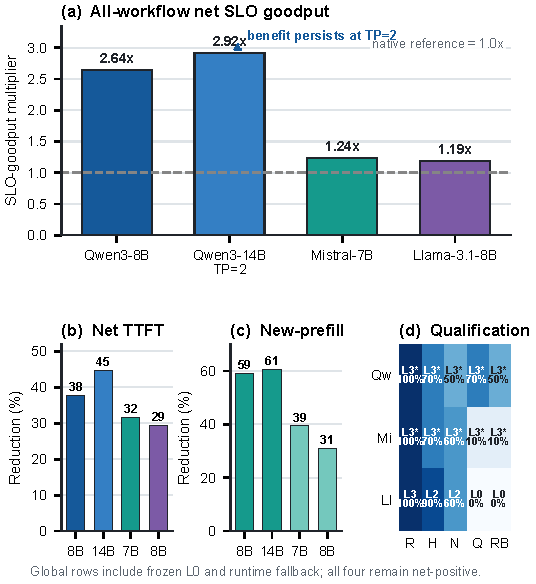
\includegraphics[width=\columnwidth]{fig2_global_benefit.pdf}
\caption{Global benefit and qualified scope. (a) Net SLO-goodput improves by 1.19--2.92$\times$. (b--c) Net mean TTFT and new-prefill work fall by 29.41--44.69\% and 30.97--60.57\%. (d) The frozen qualification map exposes model--workflow differences instead of hiding them; darker cells indicate higher certificate coverage, and L0 denotes raw order. L3* is the full compiled candidate without separately calibrated L1/L2.}
\label{fig:main_results}
\end{figure}

Qwen3-8B is the primary service platform because it supports the complete deployment matrix; Section~\ref{sec:service_perf} reports its strongest end-to-end result. Qualification yields positive global gains for every configuration across three families and two parameter scales. New-prefill reduction exceeds net TTFT reduction (e.g., 59.13\% vs.\ 37.81\% for Qwen3-8B), exposing serving and verification cost already charged by the net metric. In a same-runtime decomposition, Qwen3-8B measures 1{,}396.4~ms under raw APC, 623.0~ms with the frozen layout, and 868.4~ms with full online ContractKV; Mistral measures 1{,}102.5, 695.8, and 752.8~ms. Qwen3-14B TP=2 reaches 44.69\% net TTFT and 60.57\% prefill reduction, retaining and strengthening the measured benefit at a larger configuration without asserting a cluster-scale law.

\smallskip
\noindent\textbf{Coverage and fallback accounting.}
The global net metric includes compiled requests, runtime fallback, families prospectively frozen at L0, and verification time not hidden by slack. Thus 50\% coverage on Mistral and Llama does not mean that half of requests perform a failed verification: unqualified families route directly to L0 under the frozen manifest. Coverage is a measured model--workflow admission outcome, not an unaccounted confound. The only materially negative compiled cell is Mistral RepoBench at 10\% sparse coverage ($-2.22\%$ net TTFT); L0 remains within approximately $\pm1\%$ raw-run noise. A universal aggressive layout is therefore unsafe, whereas certification exposes each model's maximum admissible structural reuse.

% ------------------------------------------------------------
\subsection{Cross-Model Convergence on Common Scope}
\label{sec:cross_model}
% ------------------------------------------------------------

A critical question is whether ContractKV's gains are model-specific or converge under identical conditions. We answer this with a \emph{common frozen RULER scope}: 30 source-group-disjoint sessions replayed on three models under the same L3 layout, with no requalification.

\begin{table}[t]
\centering
\caption{Common frozen RULER scope: 30 identical sessions, 10 turns, 3 fresh-process pairs per model. All models consume the same sealed trace (SHA-256 committed).}
\label{tab:common_ruler}
\scriptsize
\begin{tabular}{@{}lccc@{}}
\toprule
\textbf{Metric} & \textbf{Qwen 8B} & \textbf{Mistral} & \textbf{Llama} \\
\midrule
Net mean TTFT red. & 86.64\% & 87.41\% & 85.97\% \\
\quad 95\% CI & [86.16, 87.10] & [87.06, 87.79] & [85.63, 86.29] \\
New-prefill red. & 96.71\% & 95.86\% & 95.45\% \\
SLO req/s (raw$\to$CKV) & 2.42$\to$6.33 & 2.67$\to$8.31 & 3.42$\to$14.42 \\
Goodput multiplier & 2.61$\times$ & 3.11$\times$ & 4.22$\times$ \\
\midrule
Cert.\ coverage & 100\% & 100\% & 100\% \\
Quality violations & 0 & 0 & 0 \\
Paired outputs & 810 & 810 & 810 \\
\bottomrule
\end{tabular}
\end{table}

Table~\ref{tab:common_ruler} shows close convergence: the macro TTFT reduction is \textbf{86.67\%} (95\% CI [86.44, 86.90]) and the estimates lie within 1.44 percentage points. The same sealed sessions, manifest, L3 layout, turns, and fresh-process protocol remove sample and layout asymmetry. With 100\% certified coverage, this separates \emph{model-dependent admission coverage} from the \emph{reusable-prefix mechanism}: equal certified scope yields nearly equal redundant-prefill recovery.

The SLO-goodput multiplier varies (2.61--4.22$\times$) because each model has a different raw decode rate; this reflects baseline throughput differences, not mechanism strength. As a portability check, the same offline-frozen safe layouts reduce real SGLang~0.4.9 RadixAttention TTFT by 54.93\% on Qwen and 35.53\% on Mistral. This shows that another prefix substrate can consume compiler output; it is not full online ContractKV because SGLang does not run PSTP or issue certificates.

% ------------------------------------------------------------
\subsection{Direct Comparison with Non-Prefix Reuse}
\label{sec:llama_baselines}
% ------------------------------------------------------------

Fig.~\ref{fig:llama_baselines}(a) compares alternatives on the common Llama stack. ContractKV reduces matched TTFT by 29.16\% versus CacheBlend's 26.96\%, while reducing $>0.03$ regressions from 9.956\% to 0.089\% (112$\times$); none of 1{,}125 admitted compiled requests regresses. The faster manual row (37.87\%) is an unsafe offline upper bound (1.733\% regressions). SGLang consumes an offline-frozen layout but performs neither online qualification nor PSTP.

Fig.~\ref{fig:llama_baselines}(b) localizes the tail: compiled requests have p99 899~ms and 100\% attainment at 1{,}500~ms, whereas the aggregate p99 is concentrated in deliberate L0. ContractKV is the only measured deployable row combining greater than 29\% matched reduction with zero regressions among admitted compiled requests.

\begin{figure}[t]
\centering
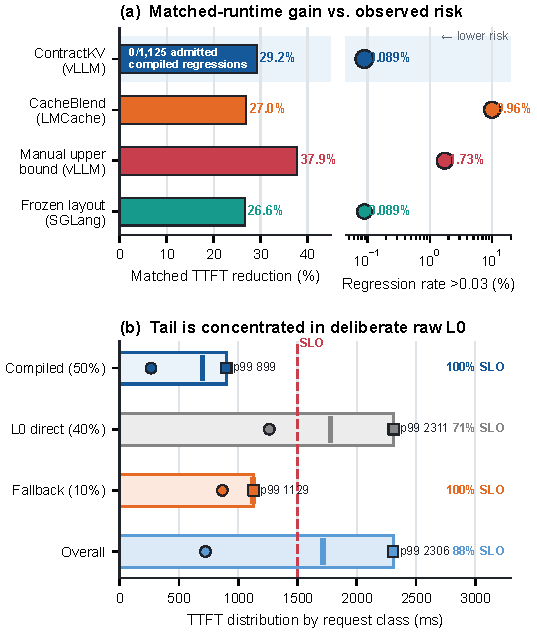
\includegraphics[width=\columnwidth]{fig3_llama_baselines.pdf}
\caption{Llama comparison and tail attribution (five fresh processes). (a) CacheBlend is slower and has 112$\times$ more regressions; manual is an unsafe upper bound; SGLang consumes only a frozen layout. (b) Bars end at p99, with mean circles and p95 ticks; the tail is concentrated in raw L0.}
\label{fig:llama_baselines}
\end{figure}

% ------------------------------------------------------------
\subsection{Service-Template Certificate}
\label{sec:certificate}
% ------------------------------------------------------------

The service-template certificate is ContractKV's most distinctive service-computing contribution. We validate it along three axes: same-engine path closure, quality preservation under fan-out, and verification amortization.

\smallskip
\noindent\textbf{Same-engine path closure.}
We replay identical five-repeat open-loop traces through D0 (native raw APC), D1 (the frozen safe layout without online verification), and D2 (full ContractKV with verifier registration and certificate publication in the serving path). Fig.~\ref{fig:verification_economics}(a--b) shows that D2 preserves D1's benefit: 500-ms SLO goodput is 1.428 versus 1.472~requests/s, mean TTFT is 194.72 versus 194.95~ms, and both have 935.86-ms p99. D2 performs four verifier registrations and four commits per process with zero failures; their wall time is charged rather than subtracted. Relative to D0, D2 improves goodput by 21.5$\times$ and reduces mean TTFT by 92.90\%, closing the earlier layout-only attribution gap.

\smallskip
\noindent\textbf{Template quality audit.}
Five deployed templates (RULER, HotpotQA, NarrativeQA, Qasper, RepoBench) are each consumed by 10 authorized tenants for 10 turns under three paired fresh processes: 1{,}350 paired future-turn executions ($5\times10\times9\times3$), clustered by template, tenant, and process. Using frozen task metrics and original budgets, we observe no raw-minus-D2 aggregate score difference, no policy violation above 0.03, no unauthorized reuse, and no scope-invalid admission. Qasper follows fail-closed raw fallback; the remaining families consume shared template certificates with no measured task-quality consequence. This audit exercises one immutable qualified template across authorized tenant/session trajectories, not merely a marker-bearing load trace.

\smallskip
\noindent\textbf{Scope-granularity ablation.}
Fig.~\ref{fig:verification_economics}(c) isolates certificate-object granularity. At identical 25-tenant locality, safe layout, and 80\% load, template scope reduces verifier calls from 125 to 5 (25$\times$), raises fan-out from 9 to 225 requests per certificate, and reduces unhidden verification cost from 25.05 to 3.24~ms/request (7.7$\times$). Serving work is unchanged: prefix-hit ratios are 97.82\% and 98.19\%, and mean TTFT, p99, and SLO goodput are statistically indistinguishable. Template scope therefore changes the economics of the safety decision, not the cache opportunity used to obtain performance.

\begin{figure}[t]
\centering
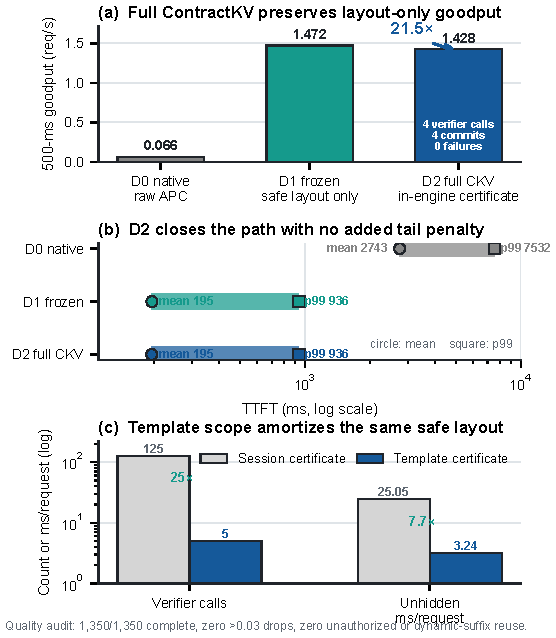
\includegraphics[width=\columnwidth]{fig4_verification_economics.pdf}
\caption{Verification closure. (a--b) Same-engine D2 preserves D1's goodput and p99; D0 is raw APC. (c) With layout/locality fixed, template scope reduces calls 25$\times$ and unhidden exposure 7.7$\times$. All 1{,}350 quality outputs complete with zero $>0.03$ drops or isolation violations.}
\label{fig:verification_economics}
\end{figure}

% ============================================================
\section{Service-Level Evaluation}
\label{sec:tsc_evaluation}
% ============================================================

We now evaluate ContractKV under multi-tenant service workloads that stress SLO goodput, consolidation density, working-set pressure, and unauthorized-reuse isolation. D0 is unmodified raw-order vLLM APC; D1 is a qualified session-scoped compiled layout; D2 is the same qualified layout with a template-scoped certificate. Arrival timestamps are generated once and replayed identically across D0/D1/D2. The unit-rate trace is exponentially distributed; 100\% load is the frozen raw-APC calibration rate, and each cell contains 1{,}125 future requests over three fresh processes. The load sweep uses Poisson open-loop arrival; the 80\% consolidation point adds the frozen ON/OFF burst overlay. Across the service study we execute 288{,}495 marker-bearing future requests, while task behavior is assessed separately on 2{,}700 task-bearing raw/ContractKV requests.

% ------------------------------------------------------------
\subsection{Service-Level Performance}
\label{sec:service_perf}
% ------------------------------------------------------------

Fig.~\ref{fig:service_locality} reports three complementary views of service-level gain.

\smallskip
\noindent\textbf{Load scaling (Fig.~\ref{fig:service_locality}a).}
Under 25-tenant service-template sharing at 80\% load and a 500-ms deadline, Qwen3-8B mean TTFT falls by 92.62\% (session-cluster 95\% CI: 91.68--93.31\%). Absolute SLO goodput rises from 0.173 to 0.831 requests/s, a gain of 0.658 requests/s (95\% CI: 0.539--0.765) and a 4.81$\times$ point multiplier. At 120\% load, raw and ContractKV goodput are 0.153 and 1.246 requests/s. A matched Mistral 25-tenant cell reduces mean TTFT by 54.35\%, p99 by 29.65\%, and new-prefill by 50.75\%, with a 0.340 requests/s absolute 500-ms goodput gain (clustered CI: 0.129--0.538). We report absolute curves rather than ratios from near-zero denominators.

\smallskip
\noindent\textbf{Consolidation density (Fig.~\ref{fig:service_locality}b).}
Across density-only rows from 10 to 80 tenants under 100\% authorized sharing, ContractKV sustains 9.41--11.07 SLO-compliant req/s while raw order remains at 0.90--1.15 requests/s. At 40 tenants, the matched density row is 1.073 versus 11.057 requests/s. A separate 40-tenant ON/OFF replay yields 1.064 versus 10.984 requests/s and raises measured Jain fairness~\cite{jain1998} from 0.666 to 1.000; we report that association without claiming a separate fairness mechanism.

\smallskip
\noindent\textbf{Physical deduplication (Fig.~\ref{fig:service_locality}c).}
At 80 tenants, peak used KV blocks fall from 530 to 149 (72\%) and free blocks rise from 1{,}856 to 2{,}237; SLO-compliant throughput is 1.152 requests/s for raw order and 11.033 requests/s for ContractKV. These are allocator-observed physical-block counts rather than a conversion inferred from new-prefill tokens. The released blocks are immediately measurable allocator headroom: a provider-specific pricing model may translate that headroom into cost or margin, but no such economic conversion is assumed here.

\begin{figure}[t]
\centering
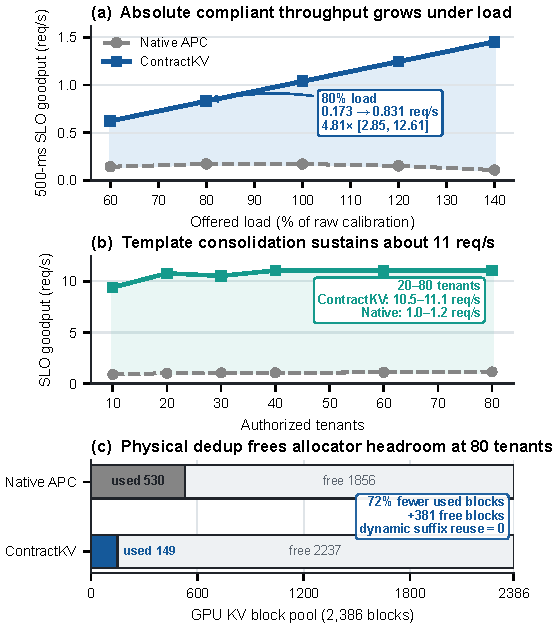
\includegraphics[width=\columnwidth]{fig5_service_locality.pdf}
\caption{Service-level benefit. (a) Absolute 500-ms SLO goodput across offered load; the shaded gap is usable compliant capacity, not a ratio with a near-zero denominator. (b) ContractKV sustains roughly 10--11 compliant requests/s across 10--80 tenants. (c) Allocator-observed peak used KV blocks fall from 530 to 149 (72\%), creating 381 additional free blocks with zero dynamic-suffix reuse.}
\label{fig:service_locality}
\end{figure}

% ------------------------------------------------------------
\subsection{Operating Region and Boundaries}
\label{sec:operating_region}
% ------------------------------------------------------------

Fig.~\ref{fig:residency} characterizes the \emph{operating region}---the conditions under which ContractKV's gains materialize.

\smallskip
\noindent\textbf{Tool-slack sensitivity.}
Using measured canary latency and live TTFT, we recompute net latency at 0, 500, 1{,}000, 1{,}500, 2{,}000, and 3{,}000~ms available slack. At zero slack, session-scoped ContractKV remains net-positive by 13.18\%, 27.26\%, and 31.20\% at concurrency 1, 2, and 4; at 2{,}000~ms the reductions are 35.99\%, 41.66\%, and 39.56\%. Thus slack expands the benefit but is not assumed free. Low-locality or short-prefix cells can still be negative, while service-template scope reduces unhidden verification to 3.24~ms/request through deployment-object fan-out.

\smallskip
\noindent\textbf{Observed sharing-ratio knee (Fig.~\ref{fig:residency}a).}
We sweep the fraction of requests authorized under a shared template over 0, 25, 50, 75, and 100\%. The measured knee lies between 50\% and 75\% sharing: once enough requests consume the certified deployment object, its prefix remains resident and TTFT reduction exceeds 85\%. This is an operating-region observation for the evaluated trace and cache size, not a universal 75\% threshold.

\smallskip
\noindent\textbf{Working-set residency (Fig.~\ref{fig:residency}b).}
Under Zipf arrival (modeling realistic skewed access), ContractKV retains 73--94\% TTFT reduction even at 50 active templates because popular templates remain cache-resident. Under round-robin arrival, gains collapse to zero when reuse distance exceeds cache capacity (25+ templates). The asymmetry confirms that ContractKV's benefit is proportional to the ratio of cache capacity to effective working-set size under the actual access distribution.

\smallskip
\noindent\textbf{Frozen net-benefit admission (Fig.~\ref{fig:residency}c).}
We freeze the admission rule on development measurements and then evaluate four held-out lanes without changing thresholds. The gate admits the 3{,}000-token/12-reuse and 5{,}000-token/10-reuse lanes; both realize positive net savings (+7.04 and +10.84~s per certificate). It routes the shorter 1{,}500-token/8-reuse and low-fan-out 3{,}500-token/6-reuse lanes directly to raw order. This is a conservative operating-point controller, not a claim of perfect benefit prediction. A separate zero-locality negative control measures 1.6--8.7\% TTFT overhead if compilation is forced, motivating the raw fallback.

\begin{figure}[t]
\centering
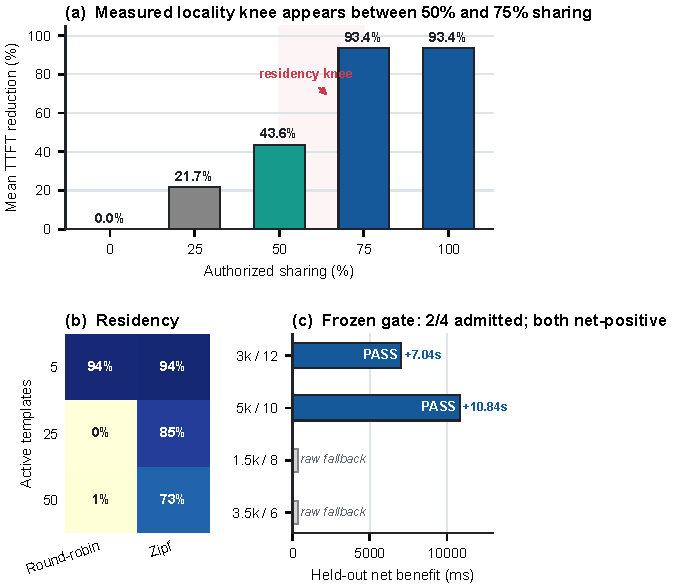
\includegraphics[width=\columnwidth]{fig6_operating_region.pdf}
\caption{Operating region. (a) The measured locality knee lies between 50\% and 75\% sharing. (b) Skew preserves hot templates as the working set grows, whereas round-robin reuse collapses beyond cache capacity. (c) The frozen net-benefit gate admits both held-out positive lanes and sends both negative lanes to raw order; bars show realized net savings per certificate.}
\label{fig:residency}
\end{figure}

% ------------------------------------------------------------
\subsection{Safety, Lifecycle, and Economics}
\label{sec:safety_lifecycle}
% ------------------------------------------------------------

Table~\ref{tab:lifecycle} consolidates the safety, lifecycle, and verification-economics evidence across all service-level experiments.

\begin{table}[t]
\centering
\caption{Safety and transactional-closure evidence. Live source-hook tests and deterministic state-machine stress are reported separately.}
\label{tab:lifecycle}
\scriptsize
\begin{tabular}{@{}p{2.55cm}p{1.35cm}p{3.55cm}@{}}
\toprule
\textbf{Dimension} & \textbf{Result} & \textbf{Evidence} \\
\midrule
Live source-hook gate & 16/16 pass & 12 commit; 4 abort; stable reuse 100\%; suffix reuse 0 \\
Concurrent fault probe & 10/10 pass & Cancel, incomplete, disconnect, duplicate, isolation \\
Signed binding stress & 15/15 pass & 0 false admit/reject; malicious metadata fails closed \\
Deterministic PSTP stress & 325{,}000 txns & 0 invariant failures; 0 aborted states with published blocks \\
Template quality audit & 1{,}350/1{,}350 & Equal aggregate score; 0 policy/isolation violations \\
Frozen benefit gate & 2/2 accepted positive & Both negative held-out lanes route to raw order \\
\bottomrule
\end{tabular}
\end{table}

The live hook establishes that PASS reaches visible shared blocks and FAIL reaches zero-pollution abort in the real scheduler path. The 325{,}000-transaction result is a deterministic in-memory concurrency closure for the formal state machine; it is not presented as 325{,}000 live GPU requests. Across lifecycle changes (model, tokenizer, policy, content, authorization, and combinations), dependent certificates invalidate before reuse and re-register under the new generation. The task-score aggregate is 0.356 for both raw and D2-template service, and Qasper remains on prospective raw fallback.

% ============================================================
\section{Related Work}
\label{sec:related}
% ============================================================

\noindent\textbf{Prefix caching substrates and serving architectures.}
PagedAttention~\cite{vllm2023} allocates KV blocks, RadixAttention~\cite{sglang2024} indexes prefixes, and Prompt Cache~\cite{promptcache2023} exposes reusable modules. CacheBlend~\cite{cacheblend2025} and SparseX~\cite{sparsex2026} recover non-prefix reuse by selective recomputation. ContractKV instead compiles a dependency-valid prefix and governs its publication; it is a control plane above these substrates. DistServe~\cite{distserve2024}, Splitwise~\cite{splitwise2024}, Mooncake~\cite{mooncake2024}, AlpaServe~\cite{alpserve2023}, TetriInfer~\cite{tetriinfer2024}, and FlexGen~\cite{flexgen2023} optimize scheduling, disaggregation, or offloading.

\smallskip
\noindent\textbf{KV reduction and prompt construction.}
H2O~\cite{h2o2023}, Scissorhands~\cite{scissorhands2023}, StreamingLLM~\cite{streamingllm2024}, SnapKV~\cite{snapkv2024}, and InfiniGen~\cite{infinigen2024} retain selected tokens, while CacheGen~\cite{llmcachegen2024} compresses transferred KV. They optimize within a fixed prompt order. Stable-first prompt construction can expose prefixes but supplies neither behavior evidence nor atomic publication. ContractKV complements both classes by increasing reusable continuity subject to a certified fallback.

\smallskip
\noindent\textbf{Service contracts.}
Classical contracts encode static QoS obligations~\cite{qosmulti2020}. ContractKV's runtime certificate authorizes sharing only for a bound model, policy, content, tenant scope, and lifecycle; mismatch fails closed. This evidence-bound service object and its transactional visibility distinguish ContractKV from application prompt engineering.

% ============================================================
\section{Discussion and Conclusion}
\label{sec:conclusion}
% ============================================================

\noindent\textbf{Why and when ContractKV helps.}
Benefit requires a large stable segment set, repeated authorized consumption, and cache residency. Fig.~\ref{fig:main_results}(d) shows that admissible reuse is a model--workflow property: RULER compiles across models, retrieval admits model-dependent levels, and order-sensitive families may freeze at L0. Always-L3 causes 10/225 development violations; prospective qualification and descent remove them. Coverage variation is thus evidence for certification, which extracts admissible reuse and preserves raw behavior elsewhere.

\smallskip
\noindent\textbf{Limitations.}
ContractKV targets repeated authorized templates; the frozen gate leaves zero-locality or negative lanes raw. Certificates are scoped empirical attestations, not proofs for arbitrary inputs. Cross-model rows charge residual verifier exposure, and the same-engine Qwen closure measures live registration/publication. PSTP is atomic within one vLLM cache domain; a disaggregated pool additionally requires distributed commit, invalidation, and recovery.

\smallskip
\noindent\textbf{Conclusion.}
ContractKV combines dependency-valid compilation, scoped certification, and transactional publication. Its strongest Qwen3-8B point reduces mean TTFT by 92.62\%, improves 500-ms SLO goodput by 4.81$\times$, and uses 72\% fewer peak KV blocks at 80 tenants. On Llama it exceeds CacheBlend's matched reduction (29.16\% versus 26.96\%) with 112$\times$ fewer observed regressions and none among admitted compiled requests. Four configurations remain net-positive with fallback charged; template certificates lower residual exposure 7.7$\times$. Failed or out-of-scope candidates publish no compiled state.

% ============================================================
% References
% ============================================================

\scriptsize
\begin{thebibliography}{99}
\setlength{\itemsep}{0pt}

\bibitem{vllm2023}
W. Kwon \textit{et al.}, ``Efficient memory management for large language model serving with {PagedAttention},'' in \textit{Proc. 29th Symp. Oper. Syst. Principles (SOSP)}, 2023, pp. 611--626.

\bibitem{sglang2024}
L. Zheng \textit{et al.}, ``{SGLang}: Efficient execution of structured language model programs,'' in \textit{Proc. 38th Conf. Neural Inf. Process. Syst. (NeurIPS)}, 2024, doi: 10.52202/079017-2000.

\bibitem{orca2022}
G. Yu, J. S. Jeong, G. Kim, S. Kim, and B. Chun, ``{Orca}: A distributed serving system for transformer-based generative models,'' in \textit{Proc. 16th USENIX Symp. Oper. Syst. Design Implement. (OSDI)}, 2022, pp. 521--538.

\bibitem{distserve2024}
Y. Zhong \textit{et al.}, ``{DistServe}: Disaggregating prefill and decoding for goodput-optimized large language model serving,'' in \textit{Proc. 18th USENIX Symp. Oper. Syst. Design Implement. (OSDI)}, 2024, pp. 193--210.

\bibitem{alpserve2023}
Z. Li \textit{et al.}, ``{AlpaServe}: Statistical multiplexing with model parallelism for deep learning serving,'' in \textit{Proc. 17th USENIX Symp. Oper. Syst. Design Implement. (OSDI)}, 2023, pp. 663--679.

\bibitem{sarathi2024}
A. Agrawal, A. Panwar, J. Mohan, N. Kwatra, B. S. Gulavani, and R. Gulavani, ``{Sarathi-Serve}: Taming the serving bubble with chunked-prefills,'' in \textit{Proc. 18th USENIX Symp. Oper. Syst. Design Implement. (OSDI)}, 2024, pp. 211--228.

\bibitem{promptcache2023}
I. Gim, G. Chen, S.-s. Lee, N. Sarda, A. Khandelwal, and L. Zhong, ``{Prompt Cache}: Modular attention reuse for low-latency inference,'' in \textit{Proc. Mach. Learn. Syst. (MLSys)}, vol.~6, 2024.

\bibitem{cacheblend2025}
J. Yao \textit{et al.}, ``{CacheBlend}: Fast large language model serving for RAG with cached knowledge fusion,'' in \textit{Proc. 20th Eur. Conf. Comput. Syst. (EuroSys)}, 2025, doi: 10.1145/3689031.3696098.

\bibitem{sparsex2026}
Q. Zhang \textit{et al.}, ``{SparseX}: Efficient segment-level KV cache sharing for interleaved LLM serving,'' \textit{arXiv preprint arXiv:2606.01751}, 2026.

\bibitem{llmcachegen2024}
Y. Liu \textit{et al.}, ``{CacheGen}: KV cache compression and streaming for fast large language model serving,'' in \textit{Proc. ACM SIGCOMM}, 2024, pp. 138--156.

\bibitem{h2o2023}
Z. Zhang \textit{et al.}, ``{H2O}: Heavy-hitter oracle for efficient generative inference of large language models,'' in \textit{Proc. 37th Int. Conf. Neural Inf. Process. Syst. (NeurIPS)}, 2023.

\bibitem{scissorhands2023}
Z. Liu \textit{et al.}, ``{Scissorhands}: Exploiting the persistence of importance hypothesis for LLM KV cache compression at test time,'' in \textit{Proc. NeurIPS}, 2023.

\bibitem{streamingllm2024}
G. Xiao, Y. Tian, B. Chen, S. Han, and M. Lewis, ``Efficient streaming language models with attention sinks,'' in \textit{Proc. 12th Int. Conf. Learn. Represent. (ICLR)}, 2024.

\bibitem{snapkv2024}
Y. Li \textit{et al.}, ``{SnapKV}: LLM knows what you are looking for before generation,'' in \textit{Proc. NeurIPS}, 2024.

\bibitem{infinigen2024}
C. Tang \textit{et al.}, ``{InfiniGen}: Efficient generative inference of large language models with dynamic KV cache management,'' in \textit{Proc. 18th USENIX Symp. Oper. Syst. Design Implement. (OSDI)}, 2024, pp. 155--172.

\bibitem{mooncake2024}
R. Qin \textit{et al.}, ``{Mooncake}: A KVCache-centric disaggregated architecture for LLM serving,'' \textit{arXiv preprint arXiv:2407.00079}, 2024.

\bibitem{react2023}
S. Yao, J. Zhao, D. Yu, N. Du, I. Shafran, K. Narasimhan, and Y. Cao, ``{ReAct}: Synergizing reasoning and acting in language models,'' in \textit{Proc. 11th Int. Conf. Learn. Represent. (ICLR)}, 2023.

\bibitem{toolformer2023}
T. Schick \textit{et al.}, ``{Toolformer}: Language models can teach themselves to use tools,'' in \textit{Proc. NeurIPS}, 2023.

\bibitem{ruler2024}
C. Hsieh \textit{et al.}, ``{RULER}: What's the real context size of your long-context language models?'' \textit{arXiv preprint arXiv:2404.06654}, 2024.

\bibitem{transformer2017}
A. Vaswani \textit{et al.}, ``Attention is all you need,'' in \textit{Proc. 31st Int. Conf. Neural Inf. Process. Syst. (NeurIPS)}, 2017, pp. 5998--6008.

\bibitem{flashattention2022}
T. Dao, D. Y. Fu, S. Ermon, A. Rudra, and C. R\'{e}, ``{FlashAttention}: Fast and memory-efficient exact attention with {IO}-awareness,'' in \textit{Proc. NeurIPS}, 2022.

\bibitem{jain1998}
R. Jain, D. Chiu, and W. Hawe, ``A quantitative measure of fairness and discrimination for resource allocation in shared computer systems,'' \textit{ACM SIGMETRICS Perform. Eval. Rev.}, vol.~26, no.~2, pp. 34--35, 1998.

\bibitem{qosmulti2020}
Y. Wang, Q. He, X. Zhang, D. Ye, and Y. Yang, ``Efficient QoS-aware service recommendation for multi-tenant service-based systems in cloud,'' \textit{IEEE Trans. Services Comput.}, vol.~13, no.~6, pp. 1045--1058, 2020, doi: 10.1109/TSC.2017.2761346.

\bibitem{tetriinfer2024}
C. Hu, H. Huang, L. Xu, X. Chen, J. Xu, S. Chen, H. Feng, C. Wang, S. Wang, Y. Bao, N. Sun, and Y. Shan, ``Inference without interference: Disaggregate LLM inference for mixed downstream workloads,'' \textit{arXiv preprint arXiv:2401.11181}, 2024.

\bibitem{flexgen2023}
Y. Sheng \textit{et al.}, ``{FlexGen}: High-throughput generative inference of large language models with a single {GPU},'' in \textit{Proc. 40th Int. Conf. Mach. Learn. (ICML)}, 2023, pp. 31094--31116.

\bibitem{longbench2024}
Y. Bai \textit{et al.}, ``{LongBench}: A bilingual, multitask benchmark for long context understanding,'' in \textit{Proc. 62nd Annu. Meeting Assoc. Comput. Linguist. (ACL)}, 2024, pp. 3119--3137.

\bibitem{splitwise2024}
P. Patel \textit{et al.}, ``{Splitwise}: Efficient generative LLM inference using phase splitting,'' in \textit{Proc. 51st Annu. Int. Symp. Comput. Archit. (ISCA)}, 2024, pp. 118--132.

\end{thebibliography}

\end{document}
